\subsection{VDCU(Vehicle Dynamics Control Unit)}
It is \gls{ecu} that manipulates torque request from driver pedal to calculate final torque for all 4 motors. The calculated torque never exceed driver request as driver request is processed as torque limitation Traction control can only decrease the total amount of requested torque.

\subsubsection{Description}
Board uses only LV and 2x \gls{can} bus.

HW :
\begin{itemize}
	\item Texas Instruments C2000 Delfino F28377 \gls{mcu}
	\item 5 V can transceiver TJA1049
\end{itemize}

\noindent SW:\\
Board is programmed using simulink embedded coder. Advantage is that we can use our developed code for IPG Carmaker simulation (MIL) directly into our formula. \gls{vdcu} uses pedal position, inertial measurement, steering wheel sensor, wheel speed sensor and motor encoders to manipulate the torque. Measurements are fed into our yaw rate control system. Output is a torque vector fed to torque vectoring algorithm that calculates the torque distribution for all wheels The resultant torque for individual wheels is lowered by traction control algorithm if needed and fed to motors.

\begin{figure}[H]
	\centering
	\includegraphics[width=\textwidth]{./img/VDCU-pcb.jpg}
	\caption{\gls{pcb} of \gls{vdcu}.}
	\label{fig:VDCU-pcb}
\end{figure}

\subsubsection{Wiring, cables}
Module is connected using headers to \gls{ecub}.

\subsubsection{Position in car}
Inside \gls{ecub} box.

\subsection {DC/DC-Converters for the car GLVS and ACP cooling fans}\label{subsec:glvs_dcdc}
Two additional DC/DC converters are present in the \gls{acp}, within the \gls{ecua}. The first DC/DC supplies the car \gls{glvs} with 24 V. The second one is the power supply for \gls{acp} cooling fans. Both DC/DC converters are of the same type, CINCON, CFB600-300S24. This type converter is an isolated type, 3000 \vac min., as per the device datasheet. (\ref{app:glvs_dcdc}). The \gls{glvs} is therefore safely isolated from the \gls{hv}, same applies for the \gls{acp} cooling system, that is also isolated from the car \gls{glvs}, due to having a separate DC/DC converter. DC/DC inputs are fused by a FU$_1$, fast blow 2 A 500 V rated fuse (\ref{app:dcdc_fuse_datasheet}).

\subsubsection{Description}

\begin{figure}[H]
	\centering
	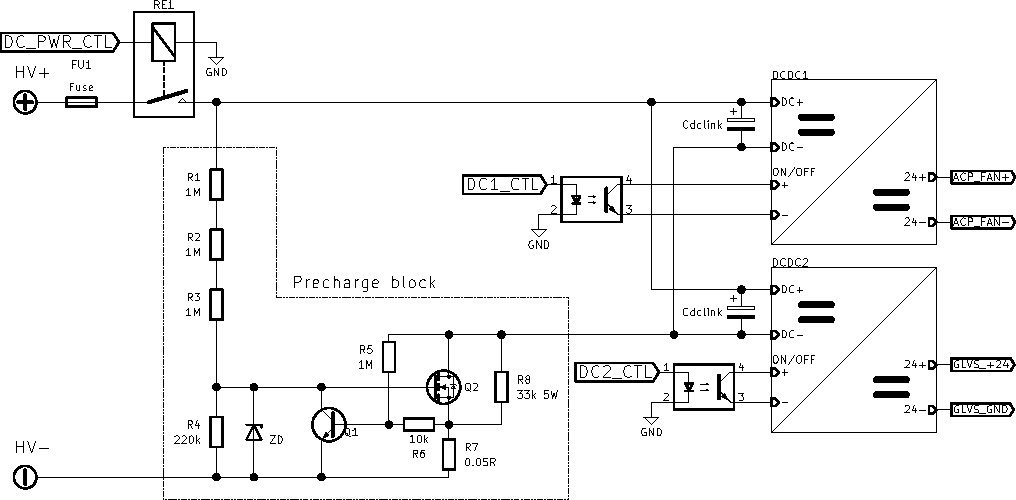
\includegraphics[width=\textwidth,clip]{./img/ECUA_DCDC_PRECHARGE.pdf}
	\caption{DC/DC pre-charge circuit and switching schematic.}
	\label{fig:precharge_dcdc_sch}
\end{figure}

Overall block diagram of the DC/DC circuitry is in \ref{fig:precharge_dcdc_sch}. Both DC/DC converters DCDC$_1$ and DCDC$_2$ share the same HV supply circuit, fused by fuse FU$_1$. Both DC/DC converters are isolated from the \gls{acp} \gls{hv} using relay RE$_1$. As additional DC link capacitors $C_{dclink}$ are required for the converters on the input HV side, a separate pre-charge circuit is also required. 
Relays type is Finder 40.52 (\ref{app:precharge_relay_datasheet}), two contacts always series connected to enhance the DC breaking capacity. Both DC/DC converters are always switched off first using their dedicated ON/OFF inputs, therefore there is no requirement for full DC current breaking capacity for the relays RE$_1$ and RE$_2$. In case of failure of one of the DC/DC converters, a fuse FU$_1$ will act to protect against further damage. 

\paragraph{Failure behavior and response}
\begin{itemize}
	\item Failure of the RE$_1$ relay in closed position only presents risk of draining the \gls{acp} charge away because of the pre-charge current and stand-by currents of both DC/DC converters. As the stand-by current of both DC/DC converters is negligible and the state of the HV circuitry of the DC/DC converters is monitored using the measurement circuitry block, the \gls{ecua} maintenance members can be notified of the failure, using the car diagnostics over the CAN bus. 
	
	\item RE$_1$ failing open presents no risk, as none of the DC/DC converters will work (\gls{acp} cooling failure, \gls{glvs} supply failure) and both the car would not be able to turn on properly and transition to the TS ON state.
	The measurement block of the DC/DC converter \gls{hv} input side is supplied using a small auxiliary isolated DC/DC converter (\ref{app:aux_dcdc_datasheet}). Signaling from the measurement block to the \gls{glvs} control side of the car is done utilizing a combination of digital signal isolator, SiLabs Si8600 series (\ref{app:ecua_isloator_datasheet}).
\end{itemize}


Both DC/DC converters DCDC$_1$ and DCDC$_2$ are fully protected against continuous overload or short circuit condition on their output, as specified in the device datasheet. Additional isolated current sense circuits are used on both converters, using a hall effect sensor, type ACS712 from Allegro (\ref{app:acs712_datasheet}). These sensors are only informative, used only for diagnostic purposes to measure current consumption from the car's \gls{glvs} system and \gls{acp} cooling.

\subsubsection{Wiring, cables}
All wiring in \gls{acp} is described in \ref{subsec:acp_wiring}.

\subsubsection{Position in car}
The DC/DC converters and all their associated circuitry are present on the \gls{ecua} \gls{pcb}. \gls{ecua} is located withing the \gls{acp} container, in a separated compartment neighbouring the \gls{air} box. Please see \ref{fig:ECUA} for details about the \gls{acp} container component placement.



